\documentclass[11pt]{amsart}
\usepackage{geometry}                % See geometry.pdf to learn the layout options. There are lots.
\geometry{letterpaper}                   % ... or a4paper or a5paper or ... 
%\geometry{landscape}                % Activate for for rotated page geometry
%\usepackage[parfill]{parskip}    % Activate to begin paragraphs with an empty line rather than an indent
\usepackage{graphicx}
\usepackage{amssymb}
\usepackage{url}
\usepackage{epstopdf}
\DeclareGraphicsRule{.tif}{png}{.png}{`convert #1 `dirname #1`/`basename #1 .tif`.png}

\title[Una paradoja en El Farol]{Una paradoja en la solución de Brian Arthur a su problema del bar El Farol}
%\author{The Author}
%\date{}                                           % Activate to display a given date or no date

\begin{document}
\maketitle

\begin{abstract}
XXXXX
\end{abstract}

\section{Introducción}
En un pequeño pueblo de 100 adultos hay un bar al que todos quieren ir cada semana. El bar abre solo una vez por semana y la experiencia que brinda cuando hay 60 o menos personas es muy agradable, pero cuando hay más de 60 personas ninguno de los asistentes la pasa bien. Si cada semana los 100 adultos deben decidir, de manera simultánea, sin una autoridad central y sin comunicación entre ellos, si ir o no al bar, ¿cómo se las pueden arreglar para aprovechar al máximo el bar? Este sencillo juego se conoce como el problema del bar El Farol, y fue propuesto por el economista Brian Arthur en 1994 \cite{Arthur1994}. Este problema ha resultado muy llamativo para distintas comunidades académicas, incluyendo la de sistemas complejos y la de física estadística, toda vez que evoca situaciones muy relevantes para la sociedad, como la distribución ecuánime de recursos limitados, la cooperación, la congestión en el uso de infraestructuras e incluso las fluctuaciones del mercado bursátil. 

La propuesta de Arthur para solucionar este problema requiere considerar una colección de reglas que predicen la asistencia futura con base en las asistencias pasadas, llamadas predictores. Cada agente tiene a su disposición un número fijo de ellos y toma su decisión con base en aquel que haya sido más preciso. Mediante simulaciones, Arthur estudió un grupo de agentes artificiales que implementan este tipo de toma de decisiones, que aquí llamaremos el \emph{método de los predictores}. Encontró que la asistencia al bar resulta cercana, en promedio, a la capacidad del bar, y que la cantidad de veces que cada agente va al bar es cercana a la cantidad justa (es decir, si son 100 rondas, la cantidad justa son 60 rondas). 

Estos resultados del método de los predictores son importantes. No obstante, varios académicos han hecho énfasis en que el análisis debe incluir también la variación de la asistencia de ronda a ronda. En efecto, a pesar de que el promedio de la asistencia está cerca de la capacidad total del bar, la asistencia fluctúa ampliamente en torno a esta de manera caótica \cite{Zambrano2004}. Como lo mostraremos más adelante, esta fluctuación deteriora notablemente el funcionamiento del sistema, especialmente si la interpretación del problema es la de congestión de infraestructura. Así pues, ¿por qué fluctúa la asistencia? ¿Es posible reducir esta fluctuación al escoger adecuadamente los parámetros del modelo o es esta una propiedad inherente al modelo?

El método de los predictores propuesto por Arthur depende esencialmente de dos variables: el tamaño $k$ de la bolsa de predictores de los agentes y el tamaño $d$ de la ventana de rondas pasadas que tales predictores pueden usar. Johnson y colegas \cite{Johnson1998} realizaron un barrido sobre $k$ -- la cantidad de predictores --, encontrando que con pocos predictores se obtiene un punto óptimo, y que al aumentar la cantidad de predictores por encima de este punto, la fluctuación aumenta también. Por su parte, Challet y colegas \cite{Challet2004} realizaron un barrido sobre $d$ -- el tamaño de la ventana de rondas pasadas --, encontrando que a medida que aumenta $d$, la fluctuación disminuye hasta un punto óptimo, por encima del cual la información se vuelve redundante. No obstante, ninguno de estos resultados considera ambos parámetros simultáneamente. Más aún, surge el interrogante de \emph{por qué} al aumentar $k$ se aumenta la fluctuación pero al aumentar $d$ se disminuye. En el presente texto explicamos por qué $k$ y $d$ tienen la influencia que tienen sobre el desempeño del sistema. 

Nuestro resultado central consiste en explicar un comportamiento paradójico inherente al método de los predictores. En efecto, dicho método favorece el uso de predictores más precisos, pero cuantos más predictores haya en la bolsa de cada agente, menos precisos se vuelven. La razón de esto es que el método en cuestión favorece la sincronía de acciones de los agentes. Esto juega en contra de la propiedad “diabólica” del problema, la cual enfatizó el mismo Arthur: “any commonalty of expectations gets broken up: If all believe few will go, all will go. But this would invalidate that belief. Similarly, if all believe most will go, nobody will go, invalidating that belief. Expectations will be forced to differ” \cite[p.~409]{Arthur1994}. Desafortunadamente, en el método de los predictores las expectativas \emph{no} tienden a diferir.

El texto está dividido en las siguientes partes. Para comenzar, puesto que las interpretaciones son variadas respecto a cómo llenar los detalles y particularidades tanto del método de los predictores como de los objetivos precisos que este debe optimizar, en \S\ref{sec:trab-rel} presentaremos brevemente las distintas interpretaciones que hemos encontrado en la literatura. Esto nos permitirá ubicar nuestra interpretación particular en el amplio espacio de opciones. En \S\ref{sec:met} presentamos nuestra implementación del método de los predictores y la definición formal de los indicadores de desempeño del sistema. En \S\ref{sec:resul} examinaremos la influencia de $k$ y $d$ sobre estos indicadores y en \S\ref{sec:parax} explicaremos por qué ellos tienen la influencia que tienen sobre la sincronía de acciones. En \S\ref{sec:disc} concluimos con una breve discusión sobre las expectativas de un método de solución a la luz de los resultados obtenidos.


\section{Trabajos relacionados}\label{sec:trab-rel}

El problema del bar El Farol ha sido muy llamativo, toda vez que evoca situaciones muy relevantes para la sociedad, como la distribución ecuánime de recursos limitados, la cooperación, la congestión en el uso de infraestructuras e incluso las fluctuaciones del mercado bursátil. No todas estas aplicaciones, sin embargo, comparten la misma estructura, por lo que no todas provienen de la misma interpretación del problema. En efecto, este requiere ser especificado en sus detalles particulares, y distintas especificaciones están relacionadas con distintas aplicaciones. La literatura sobre El Farol es variada y diversa en interpretaciones. 

\subsection{Objetivos a optimizar}
Un aspecto en el cual el planteamiento de Arthur se puede beneficiar mucho es en especificar los objetivos a optimizar. Los objetivos se especifican al definir una función de pagos. La dificultad radica en que Arthur no especificó ninguna, tal vez para enfatizar la diferencia entre su propuesta y la teoría utilitaria formalizada en la teoría de juegos. Así pues, no es de extrañar una diversidad de interpretaciones. 

La siguiente es la forma genérica de las posibles funciones de pagos $v(\mbox{acción},\mbox{aforo})$ para el problema del bar El Farol:

\vspace{-.5\baselineskip}

\[
v(\mbox{acción},\mbox{aforo}) = \begin{cases}
v_1, & \mbox{ si  acción$\,{=}\,$no ir \& aforo$\,{=}\,$congestión,}\\
v_2, & \mbox{ si  acción$\,{=}\,$no ir \& aforo$\,{=}\,$no congestión,}\\
v_3, & \mbox{ si  acción$\,{=}\,$ir \& aforo$\,{=}\,$congestión,}\\
v_4, & \mbox{ si  acción$\,{=}\,$ir \& aforo$\,{=}\,$no congestión,}\\
\end{cases}
\]

\vspace{.5\baselineskip}

La mayoría de propuestas pueden clasificarse en uno de tres tipos (compare con \cite{Chen2017}, sec. 2.2, quienes solo mencionan los últimos dos tipos de la siguiente exposición). En uno de ellos la congestión del bar es tratada como una externalidad, es decir, como una situación que afecta a todos los agentes pero que no se ve reflejada en los pagos individuales. Esta especificación se formaliza mediante una función de pagos en la cual $v_4 \geq v_3 \geq v_2=v_1$. Bajo este punto de vista, el problema es uno de distribución de recursos limitados. En efecto, cada una de las 60 sillas del bar puede ser interpretada como un recurso que los 100 jugadores quieren obtener. Este es el punto de vista bajo el que trabajan, por ejemplo, \cite{Challet2004, Ponsiglione2015}. El objetivo aquí radica en que si el bar no se llena, entonces hay recursos desperdiciados, y cuando el bar se llena, solo aquellos agentes que llegaron después no van a disponer de este recurso. Por ejemplo, Ponsiglione y colegas \cite{Ponsiglione2015} propusieron un índice, que ellos llaman Time-Box Fairness Index, que funciona parecido al coeficiente de Gini, pero que está enfocado a la idea de distribución justa de recursos. 

Otro tipo de propuestas se clasifica por una función de pagos en la cual $v_4=v_1 > v_2=v_3$. Aquí, el jugador es indiferente entre ir al bar cuando este no está congestionado o quedarse en casa cuando el bar está congestionado. Cualquiera de estos estados es preferible a los estados en los cuales el jugador o bien va a un bar congestionado o bien se queda en casa cuando el bar aún tiene capacidad. Esto implica que quedarse en casa no sea una opción segura, pero este riesgo puede traer sus beneficios. Note que este segundo tipo de función de pagos asimila el problema al juego de la minoría \cite{Challet1997}, en el cual la elección minoritaria es la ganadora. La única diferencia consiste en que en El Farol una mayoría de entre 50 y 60 agentes puede ganar al no congestionar el bar. La equivalencia entre el juego de la minoría y esta interpretación del problema del bar El Farol se da cuando la capacidad del bar es exactamente 50 agentes.

Los dos tipos anteriores difieren de un tercero, según el cual el problema es uno de congestión de infraestructura. Esto es, si el bar se llena por encima de su capacidad, todos los asistentes percibirán la situación de manera negativa y tampoco se gana si no se va al bar. Esta situación se representa mediante una función de pagos en la cual $v_4 > v_1=v_2 > v_3$, es decir, en la cual los jugadores son indiferentes a la situación del bar siempre que se queden en casa. Note que esto enfatiza la importancia que ir al bar tiene para los jugadores, toda vez que quedarse en casa nunca puede ser mejor que ir a un bar descongestionado. El problema así planteado es, en palabras del mismo Arthur, “diabólico” en varios sentidos: (i) no puede haber convergencia en comportamientos (si todos toman la misma decisión, todos pierden); (ii) la diferencia entre ambos lados del umbral en la asistencia al bar representa un salto abismal en la utilidad de los jugadores; y (iii) cuando en una ronda la utilidad es negativa, lo es para una cantidad de agentes mayor que cuando la utilidad es positiva.

En resumen, hay tres tipos posibles de interpretaciones del objetivo a optimizar: distribución de recursos, juego de la minoría, o congestión de infraestructura. En este trabajo interpretaremos el problema a resolver como del tercer tipo.

\subsection{Programas de agente}
Con esta variedad de interpretaciones no resulta sorprendente que haya también una gran variedad de programas de agente. El primer tipo que podemos catalogar es el de los agentes que adaptan su comportamiento de acuerdo a la heurística más apropiada hasta el momento, llamados best-response behavior. Lo apropiado de una heurística se ha medido o bien respecto a su \emph{precisión} -- es decir, qué tan bien la heurística ha predecido la asistencia al bar --, o al puntaje obtenido en las rondas pasadas de acuerdo a las decisiones sugeridas por la heurística. Aunque algunos trabajos han usado la segunda opción \cite{Challet2004, Chen2017}, la primera es la propuesta original de Arthur, es la más usada \cite{Arthur1994, Johnson1998, Fogel1999, Zambrano2004, Ponsiglione2015}, y es la que usamos en el presente estudio.

Otro tipo de agentes son los agentes cíclicos. Según la propuesta de Bell \& Sethares \cite{Bell2001}, un agente no predice la asistencia, sino que obedece a un parámetro que le indica la frecuencia con la que debe asistir al bar. El resultado más importante de su método de adaptación de agentes es que estos resultan divididos en dos grupos: los regulares, que van todas las rondas, y los casuales, cuya frecuencia de asistencia al bar es muy baja.

Una propuesta alternativa de programa de agente fue explorada por Fogel y colegas \cite{Fogel1999}, en la cual los predictores son funciones lineales autorregresivas sobre la asistencia en rondas pasadas, las cuales son gobernadas por un algoritmo genético de variación aleatoria y selección basada en la precisión de sus predicciones. Los autores muestran de manera convincente que la dinámica del sistema obedece a una cadena de Markov cuya dinámica no converge a un estado de equilibrio.

Uno de los programas de agente más elaborados en la literatura es el propuesto por Chen \& Gostoli \cite{Chen2017}, quienes usan redes sociales y agentes adversos a la inequidad para dirigir la dinámica del sistema para usar el bar a capacidad sin congestión, pero con una distribución justa de las asistencias de los agentes. Es importante mencionar que estos autores usan una función de pagos parecida a la del juego de la minoría y evalúan los programas de agente de acuerdo al puntaje obtenido. 

Todos los programas de agente mencionados anteriormente son deterministas. No obstante, también se han explorado alternativas estocásticas. Esto es, en lugar de usar heurísticas para decidir la asistencia al bar, los agentes usan modelos probabilísticos para tomar su decisión. El modelo más sencillo considera que cada agente $i$ va al bar con una probabilidad $p_i$. Se ha demostrado, bajo la suposición de que todos los agentes usan la misma probabilidad y que son indiferentes respecto a ir o no al bar (es decir, que la utilidad esperada de ambas estrategias son iguales), que se puede deducir una probabilidad óptima $p^*$ \cite{Franke2003, Bell2003}. Más aún, bajo el enfoque de racionalidad acotada (que, entre otras cosas, asume que los agentes no están en capacidades de deducir este óptimo), se ha explorado el método de aprendizaje por refuerzo, según el cual los agentes actualizan ronda a ronda su probabilidad $p_i$ de acuerdo al resultado de la decisión anterior. Se ha demostrado que dicho método hace converger la asistencia a la capacidad óptima sin congestión, pero divide a los agentes entre regulares, que siempre van, y casuales, que nunca van \cite{Franke2003, Bell2003}. Importante aquí es que la probabilidad nunca se actualiza cuando el agente no va al bar, de tal manera que se garantiza que algunos agentes tienden a ir cada vez menos al bar. 

\section{Métodos}\label{sec:met}

\subsection{Precisiones al modelo original}
Interpretamos el problema a resolver como uno de congestión de infraestructura. También tratamos de reproducir, de la manera más fiel posible, aunque un poco simplificada, la propuesta original de Arthur sobre el modelo de los predictores, como lo describimos a continuación.

Se tiene una población de $N$ individuos, quienes deben tomar la decisión de si acudir o no al bar, el cual tiene una capacidad $\mu N$. Usualmente, $N\,{=}\,100$ y $\mu\,{=}\,0.6$ y estos serán los valores que usaremos en nuestras simulaciones. 

En cada ronda $t$, cada agente $i$ toma una decisión $a^i_t\,{\in}\,\{0,1\}$ (donde $1\,{=}\,$ir; $0\,{=}\,$no ir) de manera independiente a los demás y todos lo hacen de manera simultánea. Denotaremos por $A_t = \sum_{i=1}^N a^i_t$ al total de acudientes al bar en una ronda dada $t$. [Si el valor de la ronda no es importante, omitiremos el subíndice $t$.] El pago para la acción de cada agente se define de la siguiente manera:

\vspace{-.5\baselineskip}

\[
v(a^i,A) = \begin{cases}
0, & \mbox{ si  $a^i\,{=}\,0$,}\\
-1, & \mbox{ si $a^i\,{=}\,1$ \& $A\,{>}\,\mu N$,}\\
1, & \mbox{ si $a^i\,{=}\,1$ \& $A\,{\leq}\,\mu N$,}\\
\end{cases}
\]

\vspace{.5\baselineskip}

La decisión de cada agente se hace mediante un predictor $s$. Al inicio del juego, cada agente escoge $k$ predictores, tomados al azar del conjunto de todos los predictores posibles. Cada uno de estos realiza una predicción de la asistencia al bar en la siguiente ronda con base en la historia de asistencias, $h_t$. Si la predicción $s(h_t)$ es menor o igual a la capacidad del bar ($\mu N$), entonces el agente va ($a^i\,{=}\,1$). De lo contrario, el agente no va. Esta historia está limitada a una cantidad $d$ de rondas. Este parámetro se conoce como la capacidad de memoria de los agentes. 

La generación del conjunto total de predictores es un aspecto del modelo que no es explícito en el artículo original. Siguiendo los ejemplos que Arthur proporciona en su texto, generamos nuestros predictores considerando, en primer lugar, dos tipos fundamentales. Estos son el promedio sobre una ventana continua de rondas y el promedio sobre una ventana cíclica de rondas, ambos dependiendo de un parámetro $w$. Por ejemplo, si la asistencia en las últimas 6 rondas ($d\,{=}\,6$) fue $h_t\,{=}\,(34, 42, 28, 54, 16, 74)$, entonces la predicción del predictor con ventana continua para $w\,{=}\,2$ es el promedio de 74 y 16, es decir, 45. Por su parte, la predicción del predictor con ventana cíclica para $w\,{=}\,2$ es el promedio de 74, 54 y 42, es decir, 56. (Observe que la ventana $w$ no puede tener una longitud superior al parámetro de memoria $d$.) En segundo lugar, para cada predictor de tipo fundamental generamos el respectivo predictor espejo, esto es, si el predictor fundamental predice $x$, entonces el predictor espejo predice $N{-}x$. El tamaño del conjunto total de todos los predictores posibles es $d\,{\times}\,2\,{\times}\,2$ (el primer valor corresponde a los posibles valores del parámetro $w$, el segundo a si es ventana continua o cíclica, y el tercero a si es fundamental o espejo).

El agente actúa, entonces, de acuerdo a lo que le sugiere su predictor más apropiado, llamado el predictor \emph{activo}, definido como aquel que ha sido más preciso durante la historia total de asistencias al bar. La precisión de un predictor, $U(s)$, la definió Arthur de la siguiente manera (aunque este resultado no aparece en el artículo original \cite{Zambrano2004}):

\vspace{-.5\baselineskip}

\[
U_t(s) = \lambda U_{t-1}(s) + (1-\lambda)\mid s(h_t) - A_t\mid
\]

\vspace{.5\baselineskip}

La función $U(s)$ siempre es mayor a cero, y es exactamente igual a cero cuando $s(h_{l})$ ha sido igual a la asistencia $A_{l}$ para todas las rondas $l\,{<}\,t$. En palabras, $U(s)$ es cero si $s$ ha predecido correctamente la asistencia en todas las rondas pasadas. Ahora bien, $U(s)$ aumenta a medida que las predicciones pasadas de $s$ se diferencian de la asistencia obtenida en la ronda correspondiente. Por esta razón, más adelante definiremos esta medida como \texttt{Inaccuracy}. Observe también que $U(s)$ depende de un parámetro $\lambda$ (con $0\,{\leq}\,\lambda\,{\leq}\,1$), el cual sirve para hacer énfasis en la última ronda (si $\lambda\,{\approx}\,0$) o en las rondas anteriores (si $\lambda\,{\approx}\,1$). Para evitar la dependencia de los resultados en este parámetro y así simplificar un poco el modelo, hemos decidido que $\lambda\,{=}\,\frac{t-1}{t}$, de tal manera que 

\vspace{-.5\baselineskip}

\[
U_t(s) = \frac{\sum_{l=0}^{t-1} \mid s(h_{t-l}) - A_{t-l}\mid}{t}
\]

\vspace{.5\baselineskip}

Finalmente, la dinámica de cada ronda es como sigue. En cada iteración, cada agente toma la historia disponible de asistencias (limitada por la capacidad de memoria $d$) para realizar una predicción mediante su predictor activo. Las decisiones de todos los agentes se combinan para determinar la asistencia al bar, la cual a su vez da lugar a los puntajes de cada agente. Con esta nueva asistencia se actualiza la historia de asistencias y la precisión de cada predictor. Luego  viene el proceso de aprendizaje, a saber, cada agente escogerá de entre las $k$ opciones en su bolsa de predictores aquel que sea más preciso. Esta dinámica se repite por $T$ rondas. En nuestras simulaciones, $T\,{=}\,100$.

\subsection{Medidas}
Observe que para cumplir el objetivo de descongestión del bar debe cumplirse que en cada ronda exactamente 60 agentes van al bar -- y así usar la infraestructura a capacidad pero evitando congestionarla. Para medir qué tanto se logró este objetivo, usamos las siguientes medidas. 

\begin{itemize}
\item[\texttt{Attendance}:] Representa la proporción de la asistencia en las últimas 20 rondas, promediada sobre 100 trials. Observe que esta medida va de 0 a 1 y es independiente de $N$.
\item[\texttt{Deviation}:] Representa la desviación estándar de la asistencia en las últimas 20 rondas, promediada sobre 100 trials.
\item[\texttt{Efficiency}:] Representa el puntaje promedio de cada agente respecto a las últimas 20 rondas, promediado sobre 100 trials.
\item[\texttt{Inaccuracy}:] Representa el promedio de $U_t(s)$ de todos los predictores activos en las últimas 20 rondas, promediado sobre 100 trials.
\end{itemize}

\section{Resultados}\label{sec:resul}
En la Figura \ref{fig:heat} se muestran los mapas de calor que se obtiene al hacer un barrido tanto de la memoria $d$ como del número de predictores $k$ en el conjunto de valores $\{1,3,6,9,12\}$. Para presentar los resultados, resulta conveniente concentrarnos primero en la familia de modelos cuyo parámetro de memoria es $d\,{=}\,1$, toda vez que las tendencias son diferentes para este valor respecto a los demás. Es importante considerar que con esta longitud de memoria sólo hay cuatro predictores en la colección total de predictores. Ahora bien, independiente del número de predictores en la bolsa de cada agente (excepto en el caso $k\,{=}\,1$), el \texttt{Attendance} está cercano a $0.5$ y el \texttt{Deviation} es altísimo y cercano a $0.5$. Esto indica que, en cada ronda, todos o ninguno de los agentes están yendo al bar, de manera completamente sincronizada. Esto es muy malo para el \texttt{Efficiency},  que es cercano a $-0.5$. El \texttt{Inaccuracy} para esta familia de modelos está cercano a 50, lo que demuestra que los cuatro posibles predictores tienen muchas dificultades con el rebote constante y extremo de la asistencia.

\begin{figure}
\begin{center}
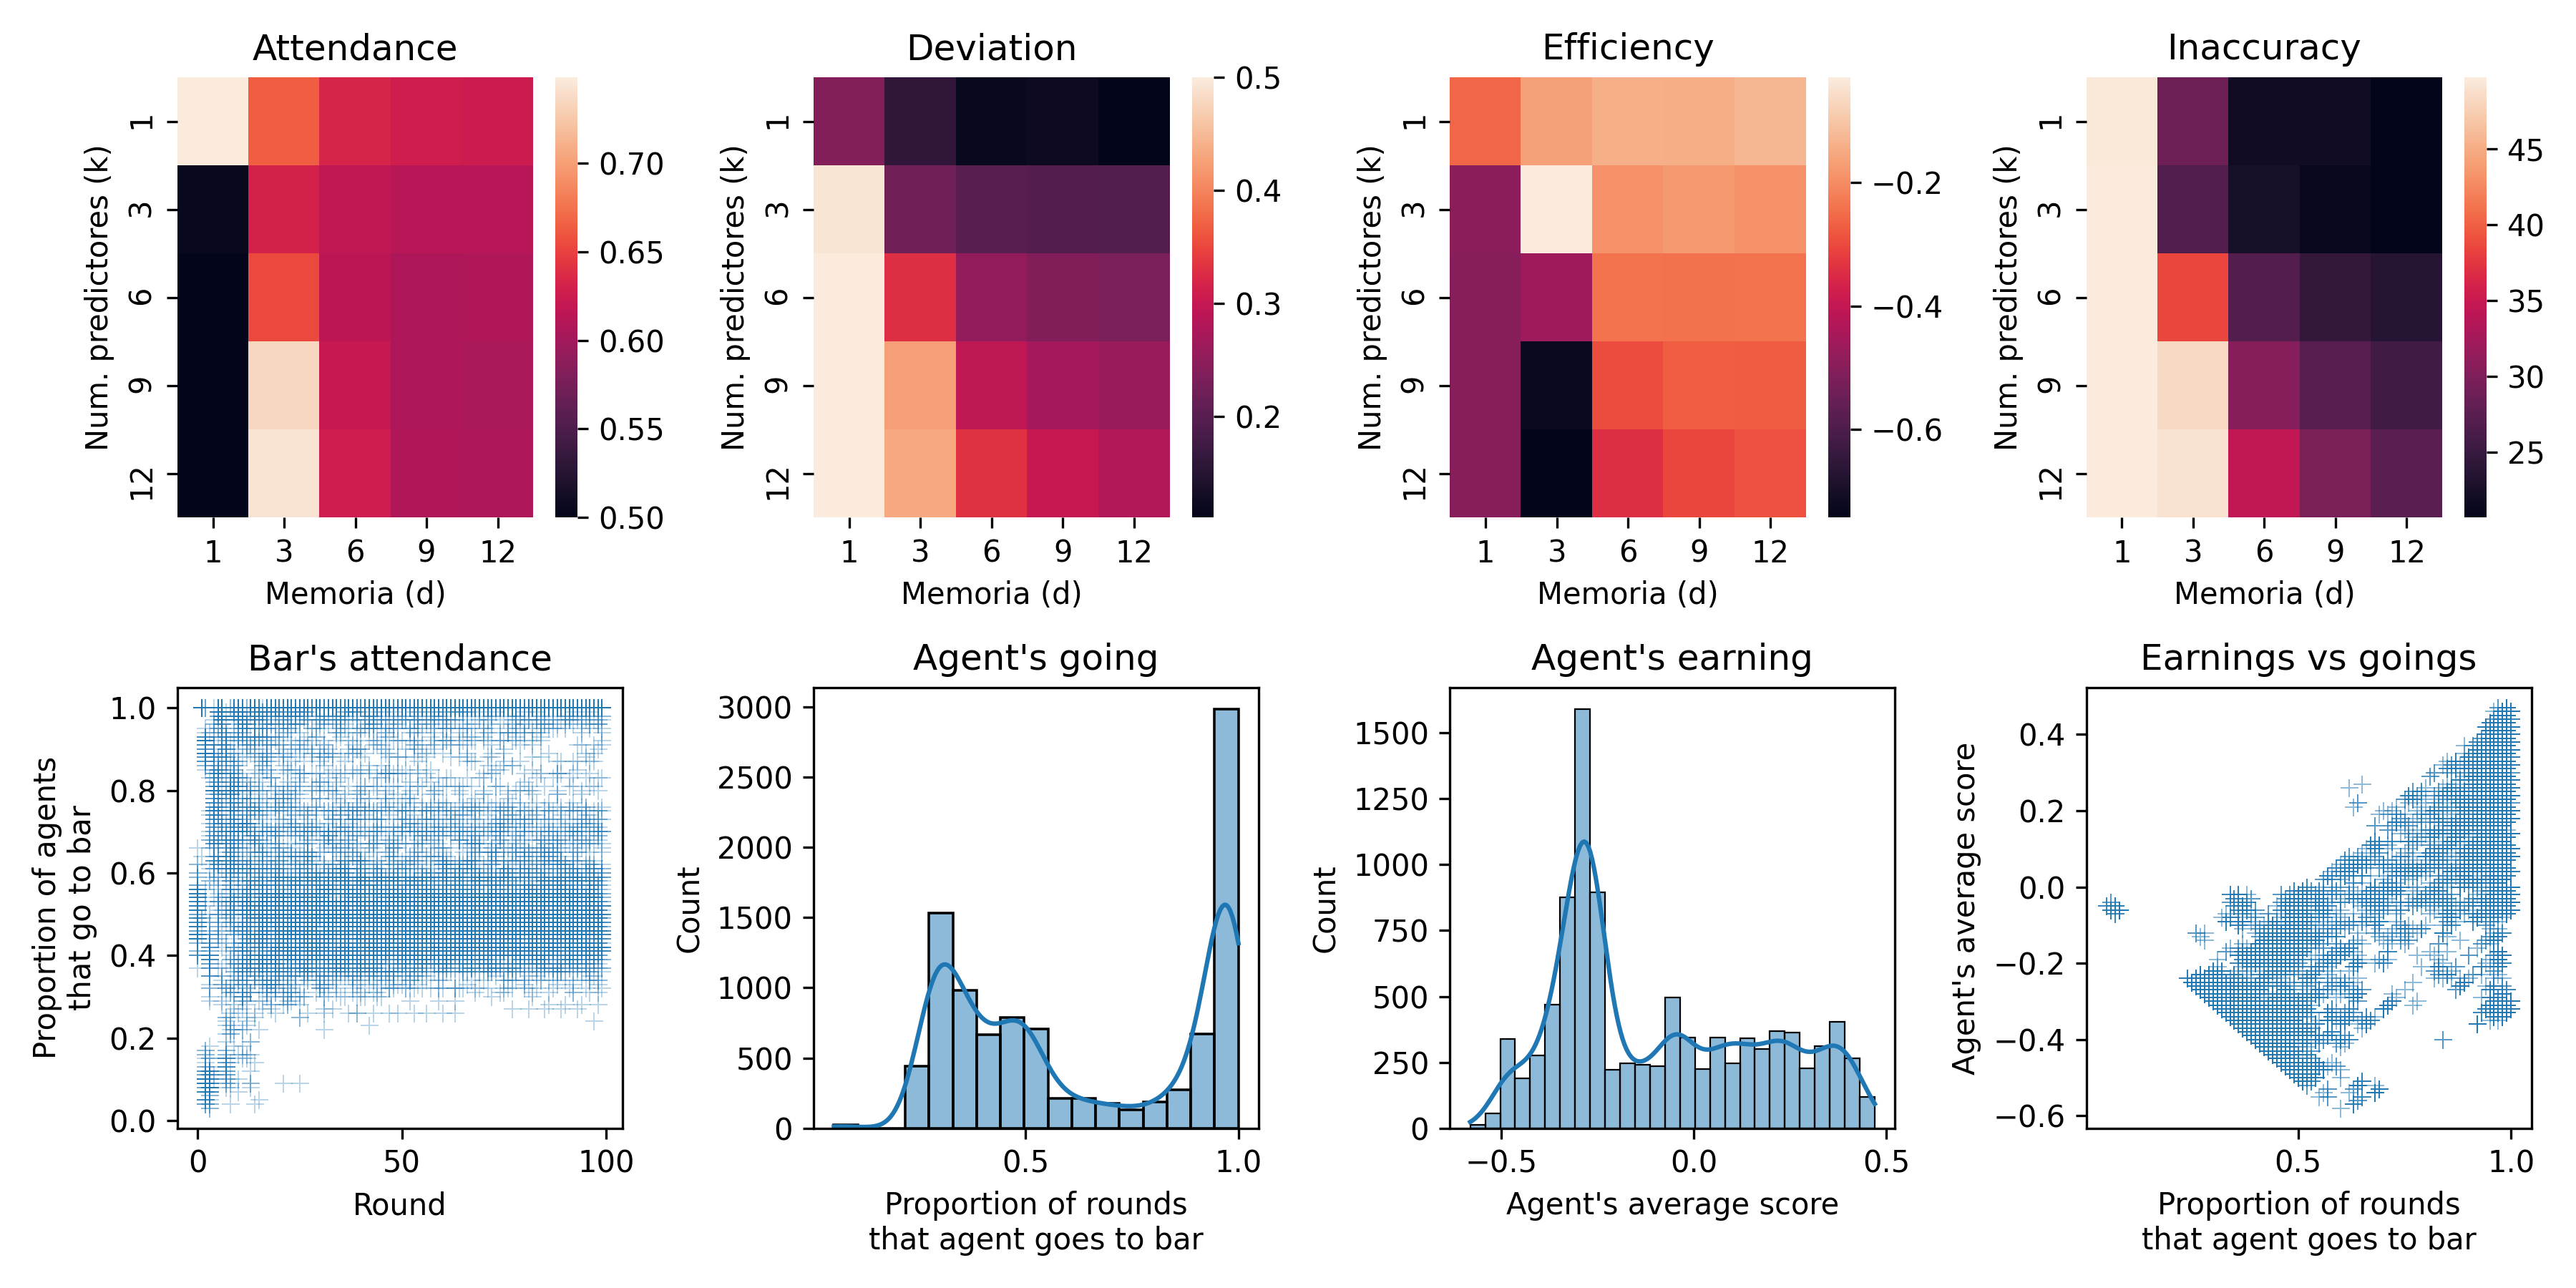
\includegraphics[width=.9\linewidth]{./Figuras/Figura1.png}
\caption{Barrido de parámetros y comportamiento del modelo óptimo. En la fila superior se presentan los mapas de calor para las cuadro medidas (\texttt{Attendance} (izquierda), \texttt{Deviation} (centro izquierda), \texttt{Efficiency} (centro derecha), \texttt{Inaccuracy} (derecha)) basados en el barrido de los parámetros $k$ (número de predictores) y $d$ (memoria o longitud de la historia) en el conjunto de valores $\{1,3,6,9,12\}$. En la fila inferior se presenta el comportamiento del modelo más eficiente, cuyos parámetros son $k\,{=}\,d\,{=}\,3$. Este comportamiento se presenta de la siguiente manera. A la izquierda se muestra la asistencia al bar por ronda, en donde cada datapoint es una ronda en alguno de los 100 trials ($\mbox{N}\,{=}\,10000$). Al centro izquierda se muestra la distribución de cuánto va (en promedio) cada agente al bar en las 100 rondas. Al centro derecha está la distribución del puntaje promedio de cada agente en las 100 rondas. Estas dos distribuciones incluyen la información de los 100 trials. A la derecha se visualiza el cruce de información entre cuánto va en promedio cada agente al bar y su puntaje promedio, en donde cada datapoint es un agente en un trial ($\mbox{N}\,{=}\,10000$).}\label{fig:heat}
\end{center}
\end{figure}

La tendencia en general (excepto para el caso $d\,{=}1$ o $\,k\,{=}\,3$) es que si se aumenta la longitud $d$ de la memoria, entonces \texttt{Attendance}, \texttt{Deviation} e \texttt{Inaccuracy} disminuyen y el \texttt{Efficiency} aumenta. Es decir, todos los parámetros mejoran. Por otro lado, si se aumenta la cantidad $k$ de predictores en la bolsa de cada agente, todas las medidas se deterioran, es decir, \texttt{Deviation} e \texttt{Inaccuracy} aumentan y el \texttt{Efficiency} disminuye (aunque \texttt{Attendance} disminuye un poco, lo cual es bueno).

En el caso particular de la familia de modelos con memoria $d\,{=}\,3$ vemos que todas las medidas tienen un pico cuando hay tres predictores ($k\,{=}\,3$), para luego deteriorarse a medida que aumentan los predictores. En efecto, la combinación de parámetros $k\,{=}\,d\,{=}\,3$ determina el modelo con mayor \texttt{Efficiency}, cuyo valor es cercano a $0$, un \texttt{Attendance} a penas por encima de $0.6$, un \texttt{Deviation} cercano al $0.25$ y un \texttt{Inaccuracy} por debajo de $30$.

COMENTAR LA FILA INFERIOR DE LA FIGURA 1

\section{La paradoja de la precisión}\label{sec:parax}

De acuerdo al método de los predictores, los agentes hacen sus predicciones mediante el predictor más preciso que tengan dentro de su bolsa de opciones. El resultado de aumentar el tamaño de esta bolsa es, como se mencionó en la sección pasada y como se muestra en la fila superior de la Figura \ref{fig:dev}, que  todas las medidas se deterioran. En particular y de manera paradójica, la precisión promedio de los predictores activos disminuye. En la fila inferior de la Figura \ref{fig:dev}, paneles izquierdo y centro-izquierda, vemos el desarrollo a través de las rondas del \texttt{Inaccuracy} de cada uno de los predictores usados por los agentes. Observe que en el modelo en el cual cada agente tiene 1 predictor los \texttt{Inaccuracy} de cada predictor son más homogéneos respecto al modelo con 12 predictores. Pero, ¿por qué disminuye la precisión y se deterioran todas las medidas a medida que se aumenta el número de predictores disponible para cada agente? 

\begin{figure}
\begin{center}
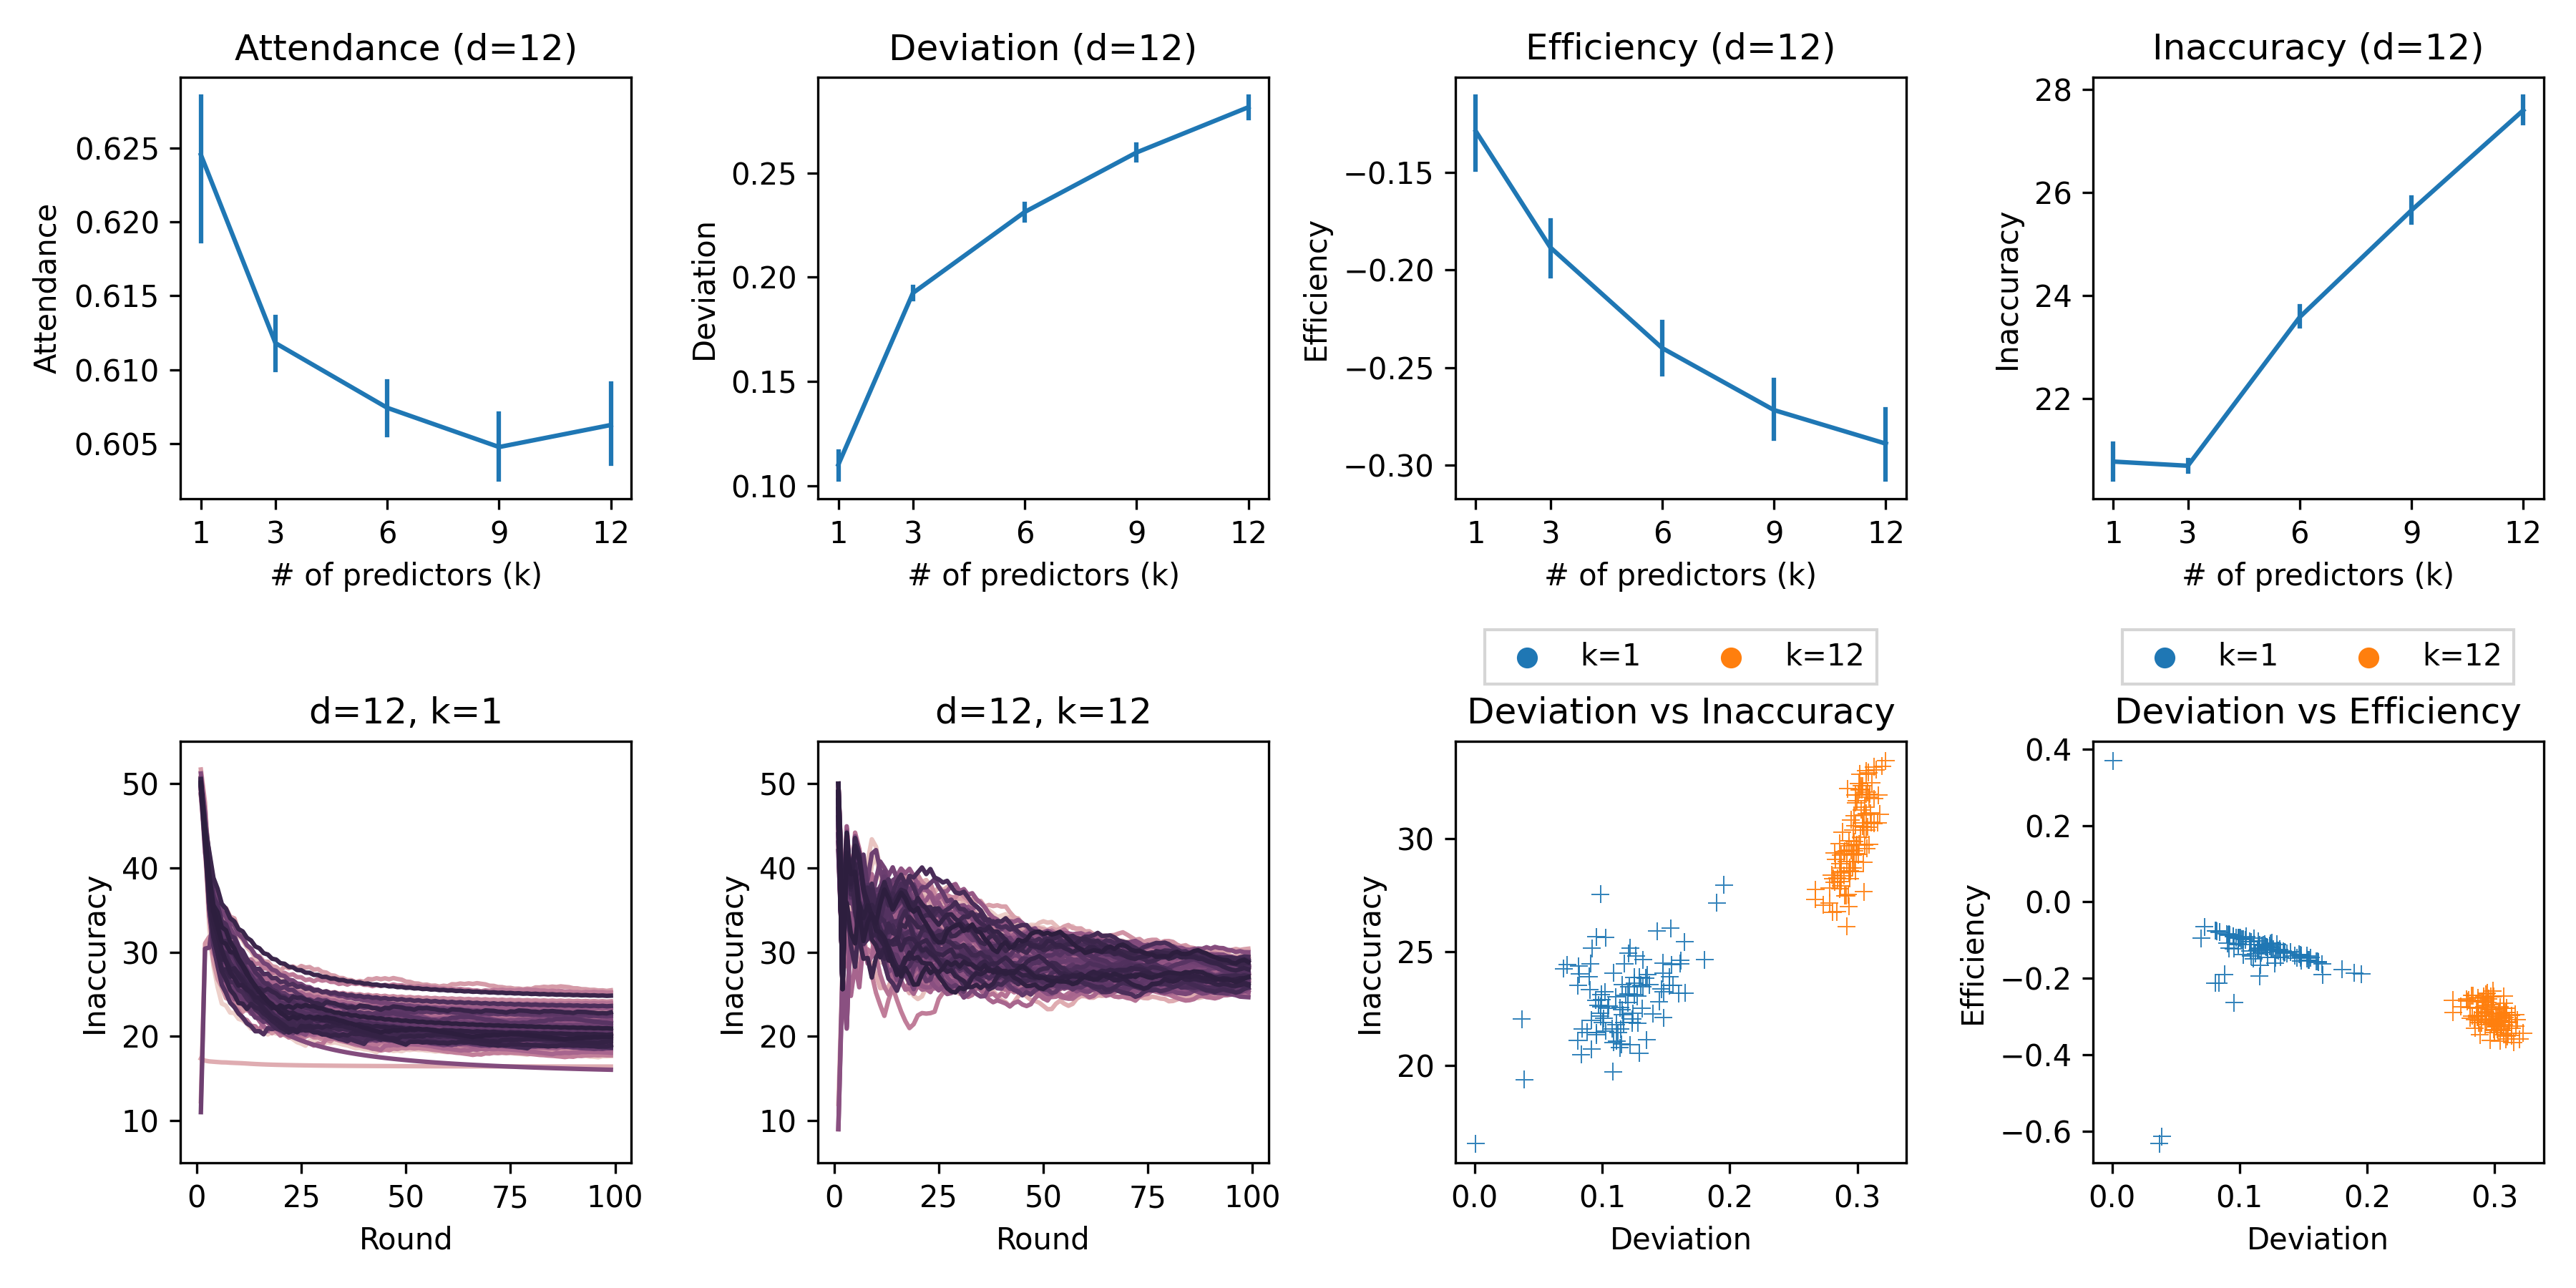
\includegraphics[width=.9\linewidth]{./Figuras/Figura2.png}
\caption{Influencia del número de predictores y el rol del \texttt{Deviation}. En la fila superior están los valores de las cuatro medidas (\texttt{Attendance} (izquierda), \texttt{Deviation} (centro-izquierda), \texttt{Efficiency} (centro-derecha), \texttt{Inaccuracy} (derecha)) al correr un modelo con memoria 12 ($d\,{=}\,12$) e ir variando el número de predictores $k$ en el conjunto de valores $\{1,3,6,9,12\}$. Las barras de error representan un intervalo de confianza del 95\%. En la fila inferior a la izquierda y centro izquierda se grafica el \texttt{Inaccuracy} contra la ronda para cada uno de los predictores del modelo, en ambos casos cuando $d\,{=}\,12$ pero con $k\,{=}1$ (izquierda) y $k\,{=}\,12$ (centro-izquierda). En las otras dos gráficas se presenta el \texttt{Deviation} contra el \texttt{Inaccuracy} (centro-derecha) y el \texttt{Efficiency} (derecha). En ambas gráficas, cada datapoint es un trial en alguno de los dos modelos con $k\,{=}1$ o $k\,{=}\,12$, diferenciados por color ($\mbox{N}\,{=}\,200$).}\label{fig:dev}
\end{center}
\end{figure}

Para desenmarañar el misterio, observe que tanto el \texttt{Inaccuracy} como el \texttt{Efficiency} están altamente correlacionados con el \texttt{Deviation}, el primero de manera directa y el segundo de manera inversa (ver Figura \ref{fig:dev} fila inferior paneles centro-derecha y derecha). La correlación es bastante alta y estadísticamente significativa en ambos casos ($\mbox{r}_{DvsI}\,{=}\,.9$, $\mbox{p}_{DvsI}\,{<}\,.001$, $\mbox{r}_{DvsE}\,{=}\,-0.676$, $\mbox{p}_{DvsE}\,{<}\,.001$). Estas correlaciones arrojan luz sobre el misterio, al mostrar que el culpable del deterioro de las medidas es, en el fondo, el \texttt{Deviation}. En lo que sigue investigaremos primero por qué aumentar el número de predictores en la bolsa aumenta el \texttt{Deviation}. Luego usaremos este resultado para explicar el aumento del \texttt{Inaccuracy} y la disminución del \texttt{Efficiency}.

\subsection{Aumento del Deviation}
Las dos hipótesis para explicar el aumento del \texttt{Deviation} son las siguientes. Aumentar el número de predictores tiene como consecuencia que:

\begin{itemize}
\item[(1)] Los agentes toman decisiones más parecidas.
\item[(2)] La mayoría de las predicciones se concentra en unas rondas por debajo de 60 y, en otras, por encima de 60.
\end{itemize}

Si estas dos hipótesis son ciertas, entonces la explicación es clara. Decisiones más parecidas implican mayor sincronía en el comportamiento de los agentes, que algunas rondas será menor a 60 (y en consecuencia la mayoría va al bar) y otras rondas será mayor a 60 (y en consecuencia la mayoría no va al bar), lo cual aumenta el \texttt{Deviation}. 

Vamos a verificar en las simulaciones si hay evidencia de (1). En la Figura \ref{fig:(1)} observemos las predicciones típicas en una ronda para cada uno de los dos modelos en cuestión. Con un predictor en la bolsa, las predicciones suelen dividirse en dos agrupamientos, mostrando distribuciones bimodales (izquierda). Por otro lado, con 12 predictores, las predicciones se aglutinan en un solo valor, mostrando distribuciones unimodales (centro). Una manera de medir este comportamiento es mediante la kurtosis de la distribución de las predicciones en cada ronda. La kurtosis mide qué tan largas son las colas de la distribución y, consecuentemente, qué tan concentrados están los valores en una distribución. En una distribución que concentra más los valores, la kurtosis será mayor. Así pues, si aumentar el número de predictores concentra las predicciones hacia un valor, entonces las kurtosis por ronda serán mayores. Esto es lo que, en efecto, se observa. En el panel de la derecha de la Figura \ref{fig:(1)} mostramos la frecuencia de las kurtosis por ronda para cada uno de los modelos, en el cual claramente se aprecia que con 1 predictor en la bolsa, la distribución de las predicciones tienen kurtosis negativas en la gran mayoría de rondas. Por otro lado, con 12 predictores hay muchas más rondas con kurtosis positivas.

\begin{figure}
\begin{center}
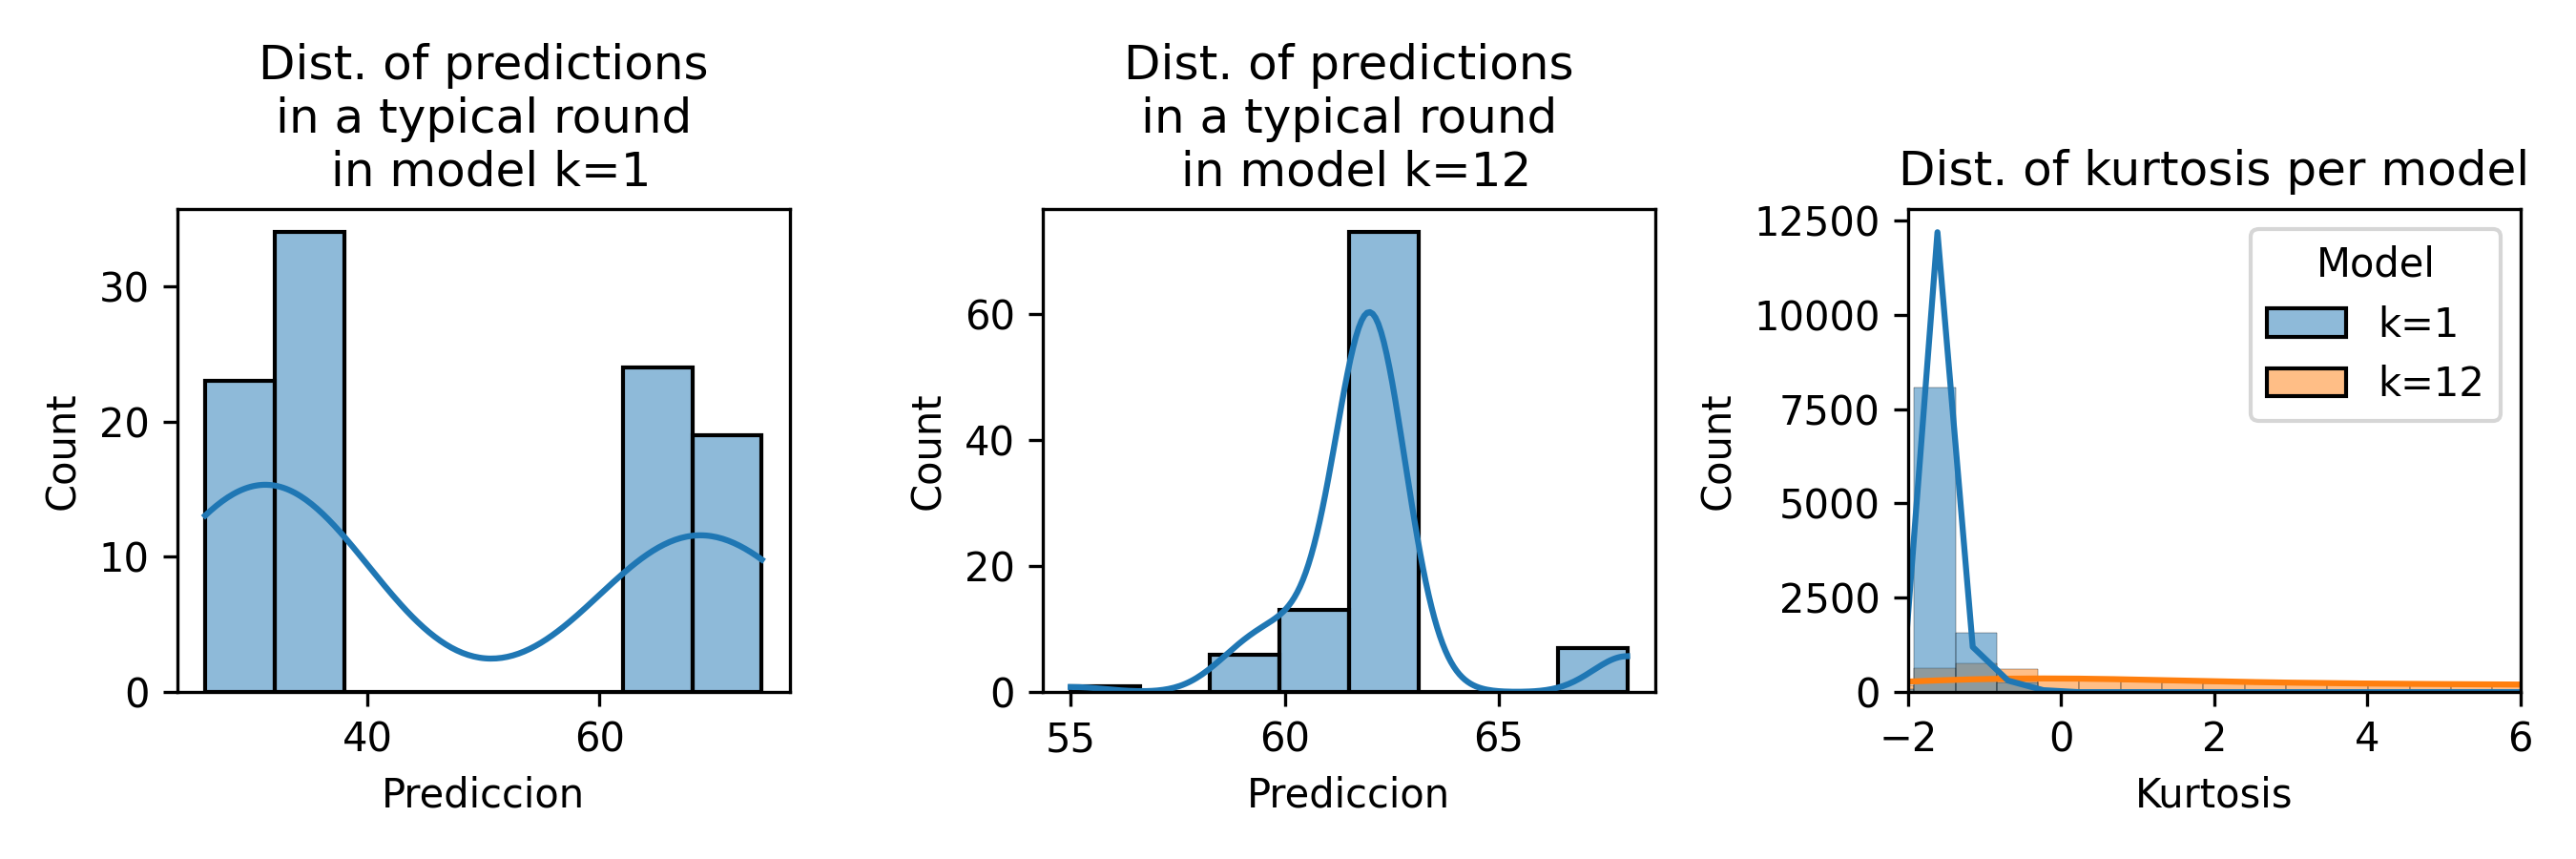
\includegraphics[width=.9\linewidth]{./Figuras/Figura3.png}
\caption{Concentración de las predicciones. EXPLICAR LA FIGURA}\label{fig:(1)}
\end{center}
\end{figure}

¿Por qué las predicciones tienden a un mismo valor a medida que aumenta el número de predictores en la bolsa? Creemos que hay tres razones para este comportamiento.

Una primera razón es que no es solo un efecto causado por usar predictores muy precisios, sino que tiene que ver con la definición misma de precisión. Dos políticas que tengan predicciones parecidas en el transcurso de las rondas, tendrán precisiones parecidas. Claro, también están aquellos pares de predictores que dan predicciones en espejo respecto a la asistencia de cada ronda y ellas también tendrán precisiones parecidas. Pero el hecho es que hay una buena probabilidad de que dos predictores con precisiones parecidas den predicciones parecidas, en especial cuando el \texttt{Inaccuracy} es pequeño.

La segunda razón está basada en la siguiente observación. Se tiene que predictores que tienden a dar valores cercanos a 60 tienden a ser más precisos. En efecto, el \texttt{Inaccuracy} es mayor para un predictor que predice 30 que para uno que predice 60 cuando la asistencia es 90. Similarmente, el \texttt{Inaccuracy}  es mayor para un predictor que predice 90 que para uno que predice 60 cuando la asistencia es de 30. Al agregar estos valores, el resultado será que los predictores que tienden a predecir una asistencia de 60 tendrán un menor \texttt{Inaccuracy}, es decir, serán más precisos. Por lo tanto, si de entre una bolsa de predictores seleccionamos aquellos que son más precisos, tendremos una mayor probabilidad de escoger uno que tienda a dar valores cercanos a 60. Este comportamiento se verifica en nuestras simulaciones, como se observa en la Figura \ref{fig:bump} a la izquierda. En esta figura, cada datapoint es una política en una ronda en alguno de los 100 trials del modelo con $d\,{=}\,k\,{=}\,12$. Los gráficos muestran el valor de la predicción que da la política en dicha ronda y la precisión que allí tiene. Se observa una tendencia según la cual las políticas más precisas son aquellas que dan una predicción cercana a 60. En el panel del centro-izquierda vemos una ronda ejemplo, en el cual los predictores más precisos son, obviamente, los predictores activos, pero todos ellos concentran sus predicciones en valores cercanos a 60. De manera general, cuanto más amplia la bolsa de predictores, los agentes predicen con base en predictores más precisos y, en consecuencia, muchas predicciones se aglutinarán en torno a valores cercanos a 60.

\begin{figure}
\begin{center}
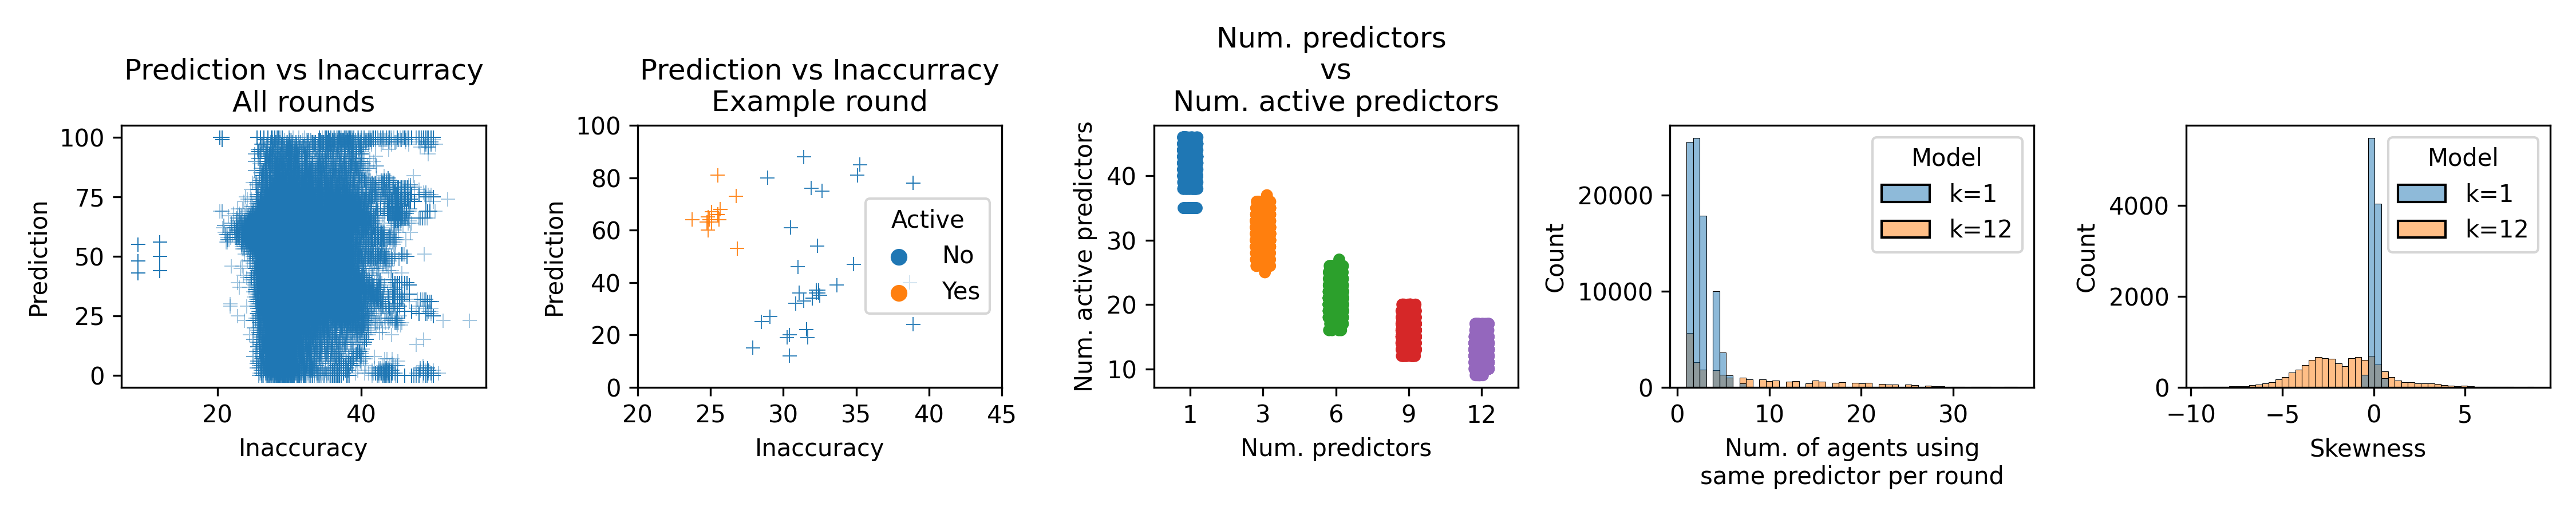
\includegraphics[width=.9\linewidth]{./Figuras/Figura4.png}
\caption{Predicción vs Inaccuracy y  aglutinación en torno a predictores activos. EXPLICAR LA FIGURA}\label{fig:bump}
\end{center}
\end{figure}

Lo tercero es que la cantidad de predictores activos disminuye a medida que aumenta la bolsa de predictores, como podemos ver en la Figura \ref{fig:bump} en el panel del centro-derecha. Esto se debe a que hay un número limitado de predictores. Cuanto más aumenta el tamaño de la bolsa de cada agente, más predictores van a compartir. En efecto, como se ve en el panel de la derecha de la Figura \ref{fig:bump}, la cantidad de agentes compartiendo la misma política en cada ronda es mucho más grande con 12 predictores en la bolsa que con 1 predictor. Adicionalmente, considere que varios de esos predictores resultarán muy precisos, por lo que las predicciones que los agentes harán con base en ellos serán muy parecidas. 

Con estos argumentos también es fácil ver por qué (2) es cierta, es decir, por qué una gran cantidad de predicciones se concentran por debajo de 60 en algunas rondas y en otras por encima. Hemos visto que las predicciones se concentran cerca a 60, pero no exactamente en 60. Para ver que estas predicciones no se distribuyen simétricamente en torno a 60, podemos considerar el skewness de la distribucción de predicciones. Como se ve en la Figura \ref{fig:bump}, cuando cada agente tiene 12 predictores, el sesgo por ronda cambia de positivo a negativo, sin aglutinarse en el 0, como lo hace en el modelo donde cada agente tiene 1 solo predictor.

\subsection{Aumento del Inaccuracy}
1. Predicciones tienden a 60.
2. Aumento del Deviation.

(1) y (2) implican aumento del Inaccuracy, toda vez que los predictores tienden a predecir un número cercano a 60, pero las asistencias tienden a los extremos.

\subsection{Influencia de la memoria}

AQUÍ HAY QUE EXPLORAR ESTO Y DECIR ALGO DE POR QUÉ LA MEMORIA MEJORA LAS MEDIDAS.

\section{Discusión}\label{sec:disc}

CONCLUIR

\bibliographystyle{vancouver}
\bibliography{BibElFarol.bib}

\end{document}  